\begin{frame}[standout]
	Generating Counterfactual Explanations
\end{frame}


\begin{frame}{Construction}
	\begin{center}
		\includegraphics[width=0.7\textwidth, page=2]{graphics}
	\end{center}


	\begin{center}
		\begin{tabular}{cc}
			$
			f(x) = \sigma \left ( \beta^T NN(x) \right) \qquad \qquad
			$ &
			$
			f^\dagger(y) = NN^{-1}\left( f(x) - \frac{\langle f(x), \beta\rangle \beta}{||\beta||}\right)
			$
		\end{tabular}
	\end{center}
\end{frame}

\begin{frame}{Properties and Extensions}
	\begin{center}
	    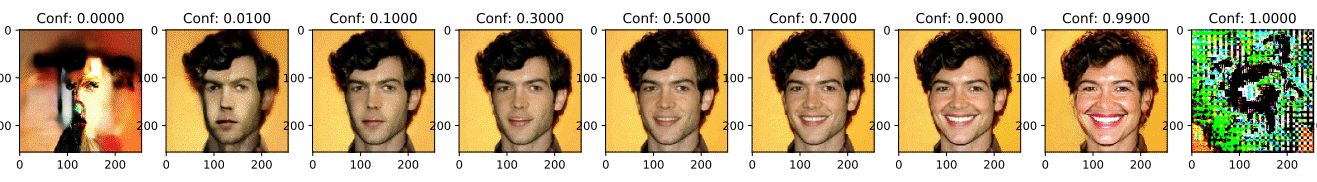
\includegraphics[width=\textwidth]{interpolation.png}
	\end{center}

	\begin{columns}
		\begin{column}{0.5\textwidth}
			\alert{Properties}
			\begin{itemize}
				\item \alert{First} ``one-evaluation-solution'' (Fast)
				\item Built to produce counterfactual explanations
			\end{itemize}
		\end{column}
		\begin{column}{0.5\textwidth}
			\alert{Extensions}
			\begin{itemize}
				\item Training $NN$ and $\beta$ jointly
				\item Evaluating Counterfactual explanations
				\item Bound difference in $X$ from change in $Z$ space
					\begin{itemize}
						\item Lipschitz constraint on $NN$
					\end{itemize}
			\end{itemize}
		\end{column}

	\end{columns}
	\vspace{1em}
	$$
		Score(X, \hat X) = ||\Delta_X||_1 + vec(\Delta_X)\rL vec(\Delta_X) + \boldsymbol{1}_{f(\hat X) \neq \bar f(\hat X)}
	$$
\end{frame}

